\section{Authentication}

\subsection{Configuration}

Configuring Auth0 to serve an SPA is fairly painless; the
only constraint is asymmetric encryption is required for
signing the authentication tokens, as a SPA cannot store
secrets in browser.
Once set to use RS256, the only remaining configuration was
to disable all authentication mechanisms other than
socials.

In the frontend, the authentication flow utilises the SDK
offered by Auth0 for Vue 3, requiring the provider's
domain, client\_id, and audience which is stored in
environment files: 

\begin{figure}[H] 

  \centering 

  \small 

  \lstinputlisting{06 development/assets/auth0 sdk.ts}

  \caption{Configuring Auth0 Vue SDK} 

\end{figure} 

It provides helper methods, such as
\lstinline{loginWithPopup} and
\lstinline{getAccessTokenSilently}, and flags like
\lstinline{isAuthenticated}, used before directing to
authenticated pages in a navigation guard.

To send authenticated API requests, the access token is
send using the standard \lstinline{Bearer} schema.
It is verified using the \gls{jwks} exposed by Auth0 via
Microsoft's \lstinline{JwtBearer} package.

\begin{figure}[h]
  \centering

  \begin{subfigure}{\subfigwidth}
    \centering
    \frame{\includegraphics[width=0.9\linewidth]{06
        development/assets/auth flow/home page no
        auth.png}}
    \caption{Home page before authenticating}
  \end{subfigure}
  \begin{subfigure}{\subfigwidth}
    \centering
    \frame{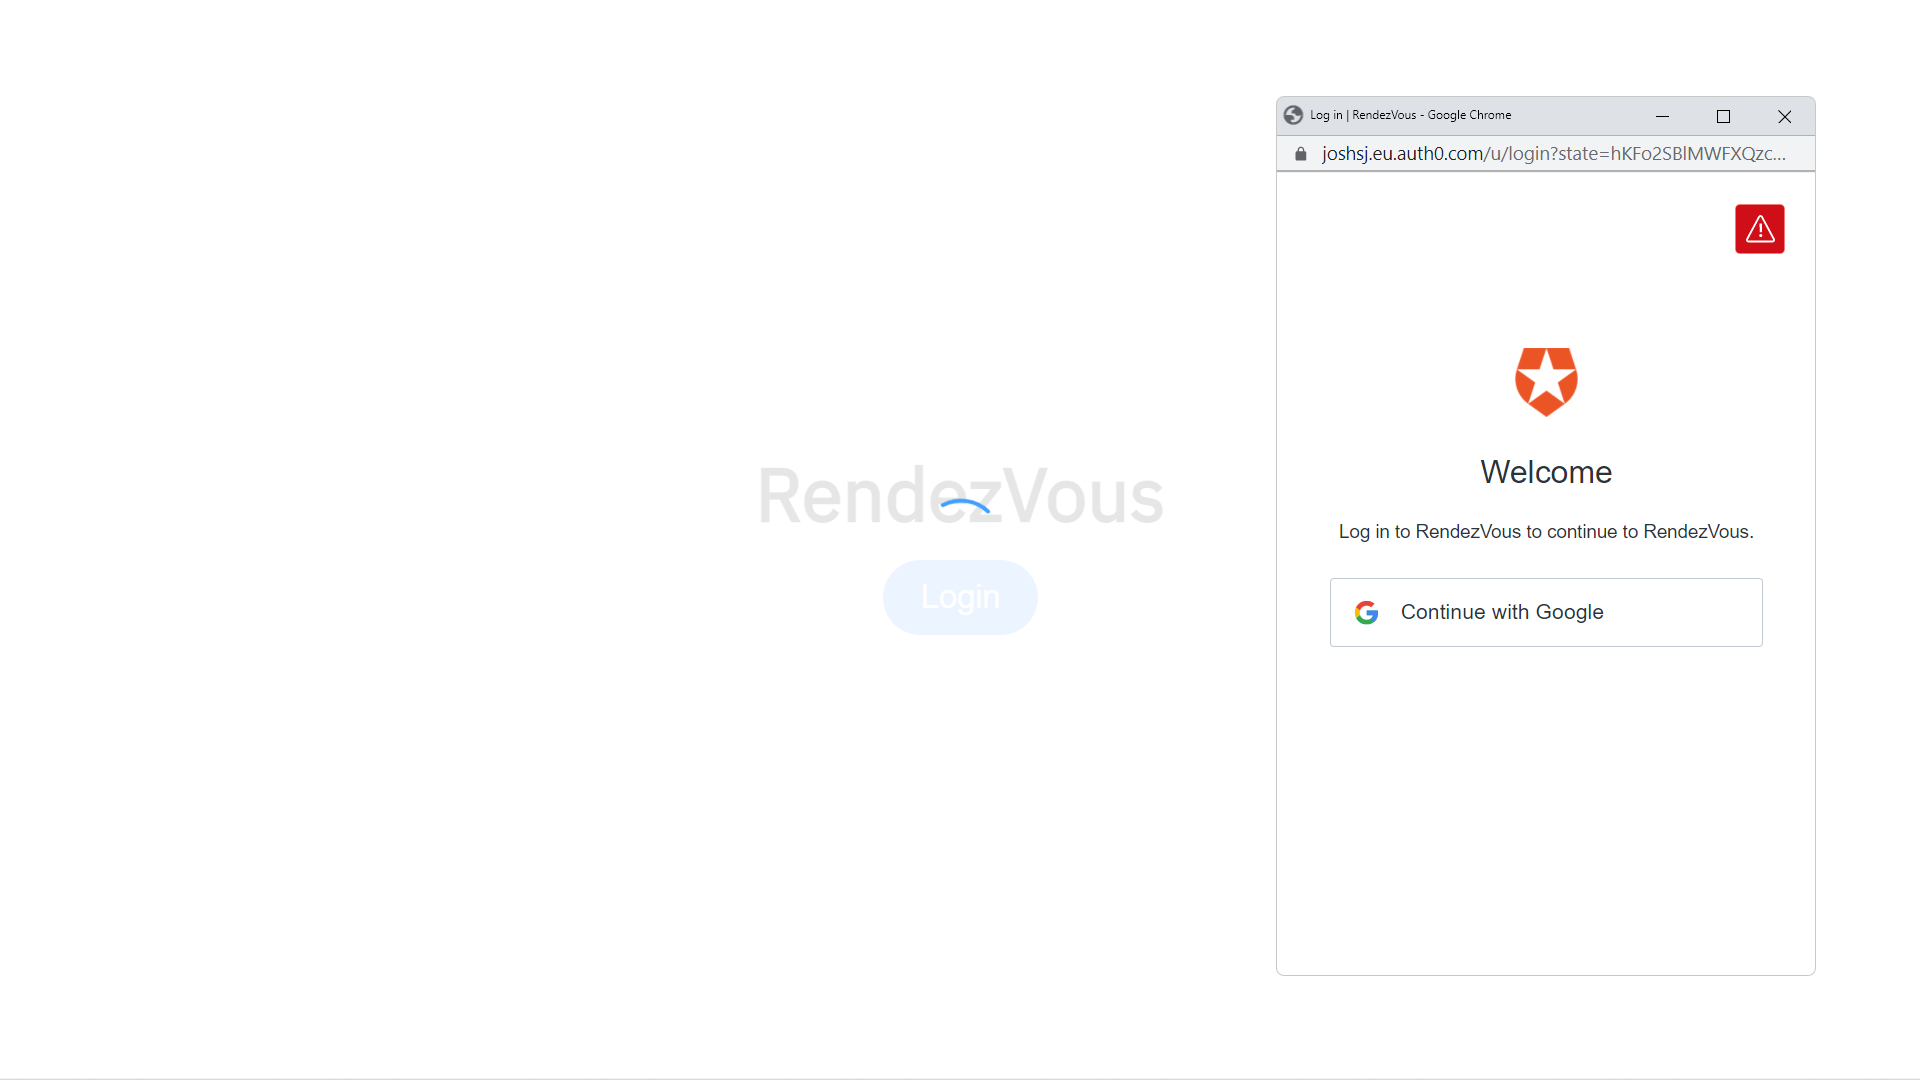
\includegraphics[width=0.9\linewidth]{06
        development/assets/auth flow/auth popup.png}}
    \caption{Authentication Popup}
  \end{subfigure}
  \begin{subfigure}{\subfigwidth}
    \centering
    \frame{\includegraphics[width=0.9\linewidth]{06
        development/assets/auth flow/home page with
        auth.png}}
    \caption{Home page after authenticating}
  \end{subfigure}
  \begin{subfigure}{\subfigwidth}
    \centering
    \frame{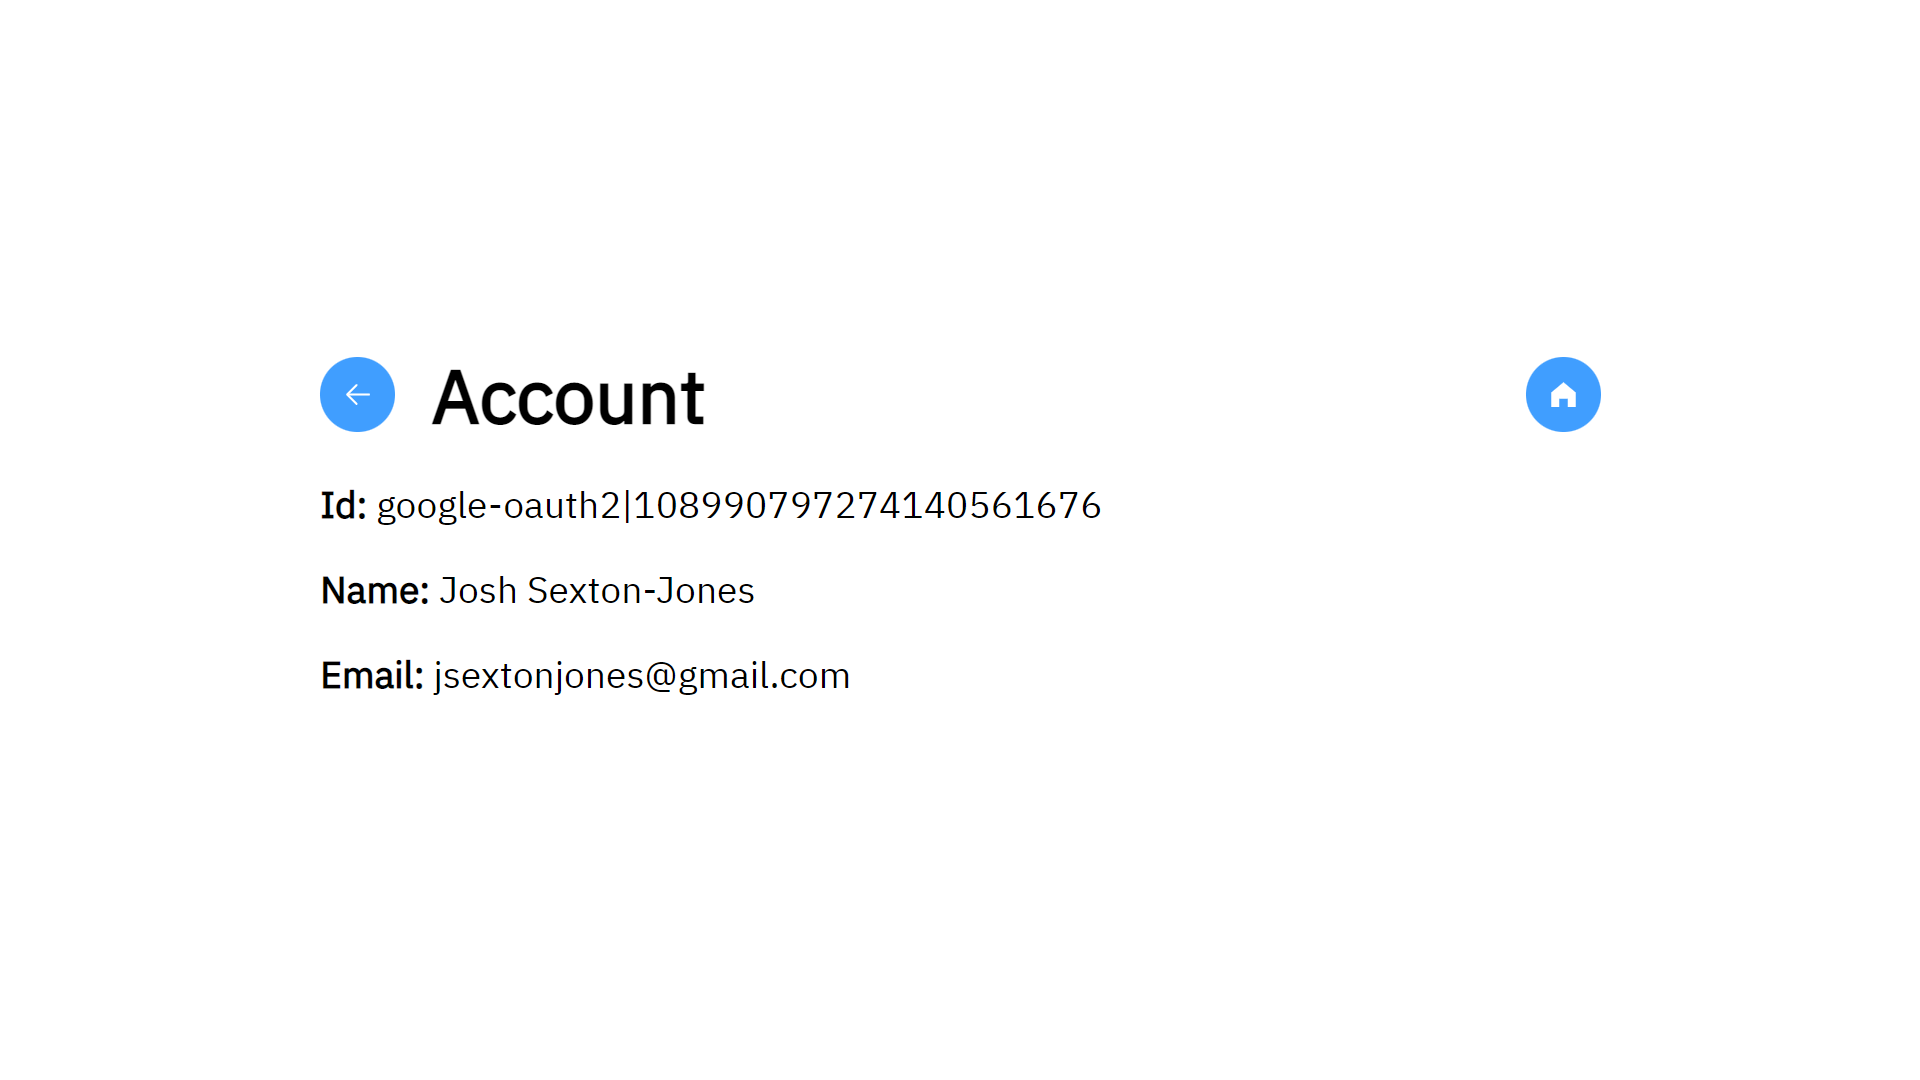
\includegraphics[width=0.9\linewidth]{06
        development/assets/auth flow/account page.png}}
    \caption{Account page}
  \end{subfigure}

  \caption{Frontend Authentication Flow}
  \label{fig:authFlow}
\end{figure}

\subsection{Saving Employee Information}

To persist users in the database, the user's required
information must be included in the access toke.
By default, Auth0 only stores their ID, so a custom
\enquote{Rule} is required to add additional claims.

As seen in Figure \ref{fig:userInfo}, the API updates the
user in the database using these claim before each API
request is executed, ensuring their information is always
up to date.

\begin{figure}[h]
  \centering
  \small
  \begin{subfigure}{\linewidth}
    \lstinputlisting{06 development/assets/user
      info/additional claims action.ts}
    \caption{Setting additional claims in Auth0}
  \end{subfigure}
  \begin{subfigure}{\linewidth}
    \lstinputlisting{06 development/assets/user info/upsert
      action filter.cs}
    \caption{Persisting the additional employee
      information}
  \end{subfigure}

  \caption{Saving user information from an access token}
  \label{fig:userInfo}
\end{figure}
